\documentclass{article}
\usepackage[T1]{fontenc}
\usepackage{lmodern}
\usepackage{graphicx}
\usepackage{amsmath,amssymb}
\usepackage[a4paper,margin=2cm]{geometry}
\usepackage[absolute,overlay]{textpos}
\setlength{\TPHorizModule}{1mm}
\setlength{\TPVertModule}{1mm}
\usepackage[indonesian]{babel}
\usepackage{hyperref}
\setlength{\emergencystretch}{2em}
% unit: Halaman 34

\begin{document}

% === Halaman 34 (llm) ===

\vspace{231.07mm}

\begin{center}
\Huge Efek longsoran di dalam DES \\
\Large (mengubah satu bit kunci)
\end{center}

\vspace{10mm}

% deskripsi: Tabel yang menunjukkan efek longsoran (avalanche effect) pada algoritma DES, membandingkan nilai state internal antar round ketika satu bit kunci diubah, disertai dengan nilai delta ($\delta$) yang mengukur perbedaan bit.
% bbox normalisasi: [0.1930, 0.1850, 0.7430, 0.9630]
\begin{textblock*}{115.50mm}(40.53mm,54.95mm)
\noindent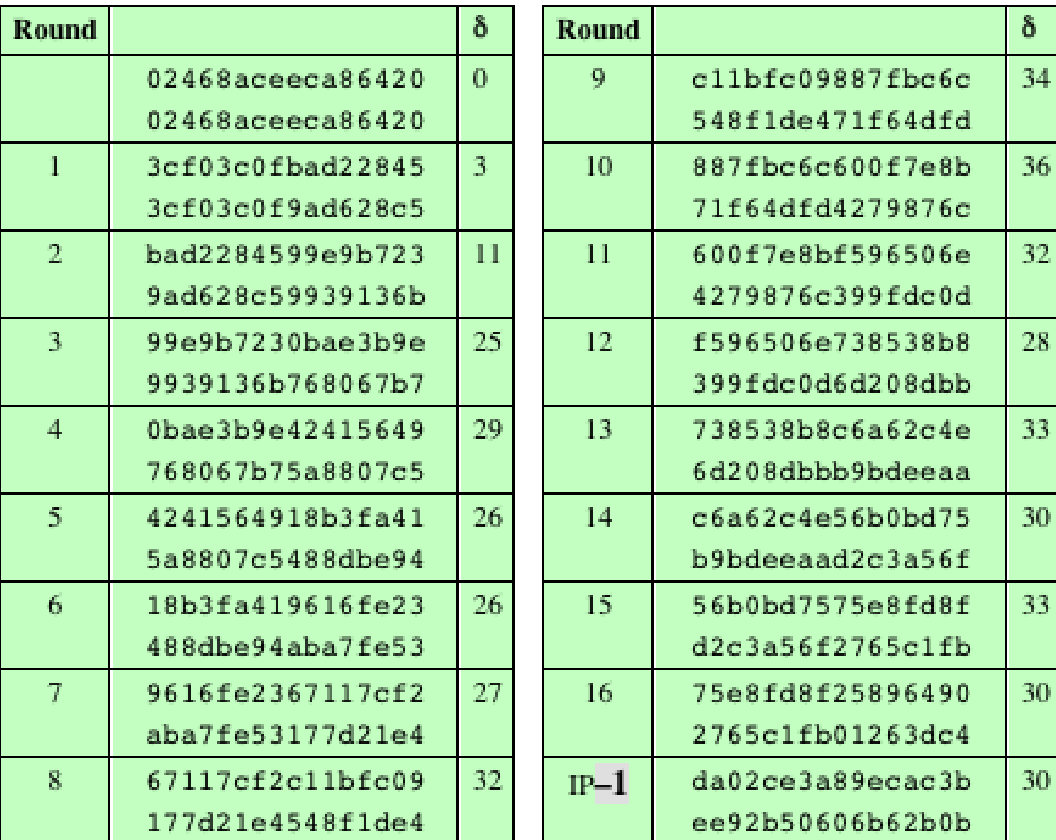
\includegraphics[width=115.50mm,height=231.07mm]{../../images/llm/page_034_img_01.png}%
\end{textblock*}

\end{document}
